\chapter{Cartesian Grids of Kernel Functions and Orthonormalization}\label{sec:grids}

In this work, we use Cartesian grids as dictionaries for kernel least-mean-square filters. Cartesian grids are grids of points disposed in the space as the vertices of squares, cubes or hypercubes, whose edges are parallel to the system axes. 

\section{Cartesian Grids}

Usually, kernel filters use ad-hoc dictionaries \cite{engel_kernel_2004,richard_online_2009,platt_resource-allocating_1991,badong_chen_quantized_2012,bueno_gram-schmidt-based_2020}, that is, the dictionary is created as the input vectors arrive and in the order they arrive. This depends on the input vector distribution and may cause problems if outliers arrive, since outliers usually are put on the dictionary, causing more computation than should be needed. Also, even after orthonormalization, as in the case of the GS-KLMS, different realizations of the process that generates the input vectors could result in different dictionaries, and may even lead to the Mean Squared Error to have a different behavior. 
Figure \ref{fig:err2_sparsifications} shows four the Mean Square Error of 10 realizations of a KLMS with different sparsification techniques (Novelty Criterion, Coherence Criterion, Gram-Schmidt and the Cartesian Grid proposed in this work). It is possible to see that the Cartesian Grid have smaller variation of the MSE in steady state between realisations.
%\textcolor{red}{Put figure showing the MSE for different realizations and with different sparsification methods.}
\begin{figure}
    \centering
    \begin{subfigure}[b]{0.45\linewidth}
        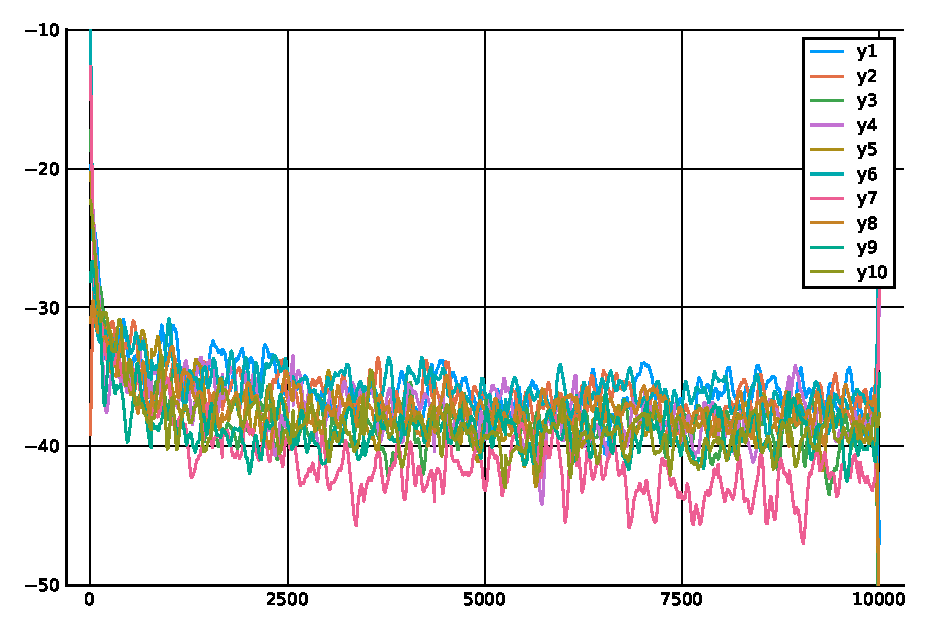
\includegraphics[width=\linewidth]{figuras/err2_nc_sparse.eps}
        \caption{}
        \label{fig:err2_nc}
    \end{subfigure}
    \begin{subfigure}[b]{0.45\linewidth}
        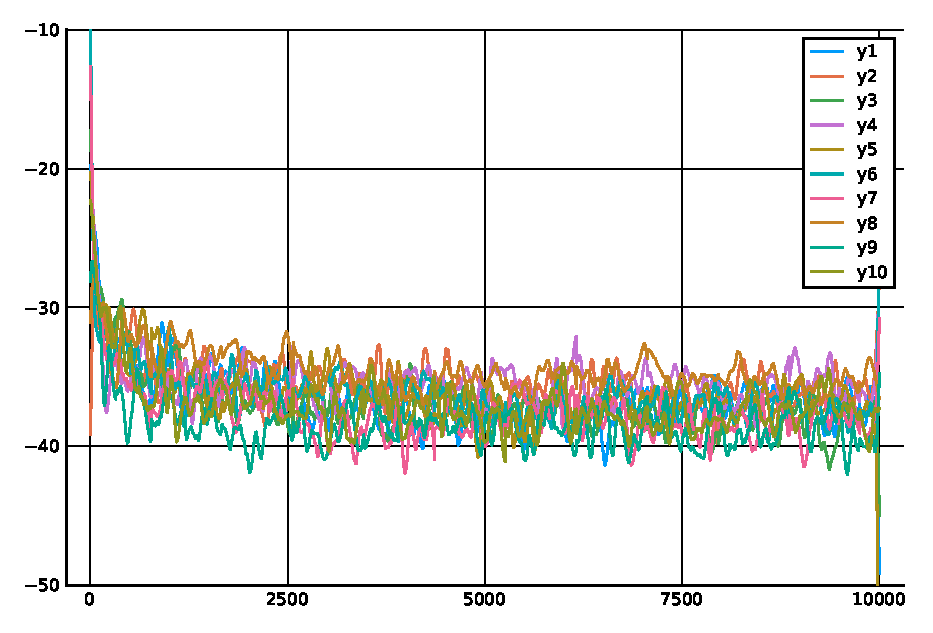
\includegraphics[width=\linewidth]{figuras/err2_cc_sparse.eps}
        \caption{}
        \label{fig:err2_cc}
    \end{subfigure}
    \begin{subfigure}[b]{0.45\linewidth}
        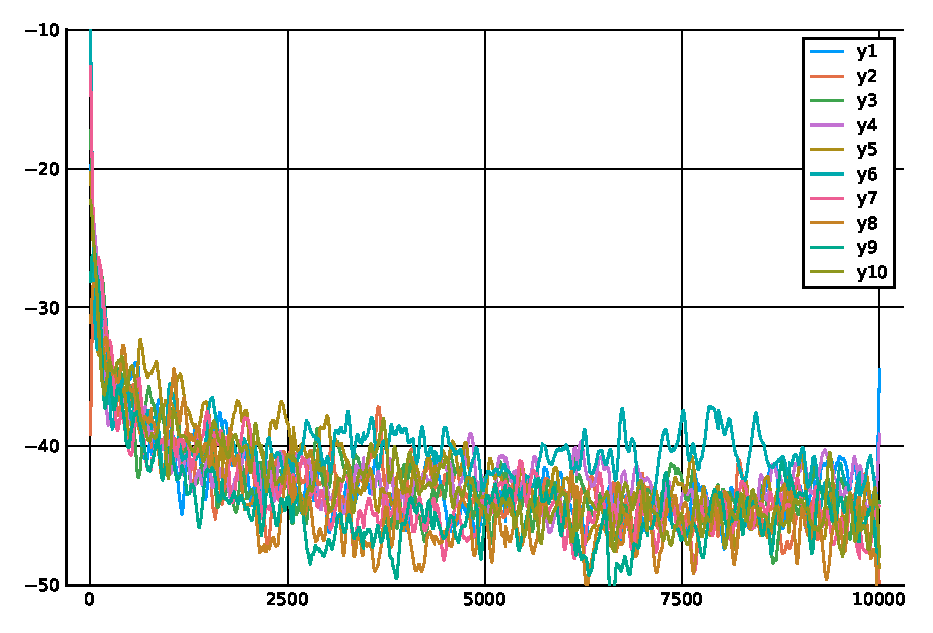
\includegraphics[width=\linewidth]{figuras/err2_gs_sparse.eps}
        \caption{}
        \label{fig:err2_gs}
    \end{subfigure}
    \begin{subfigure}[b]{0.45\linewidth}
        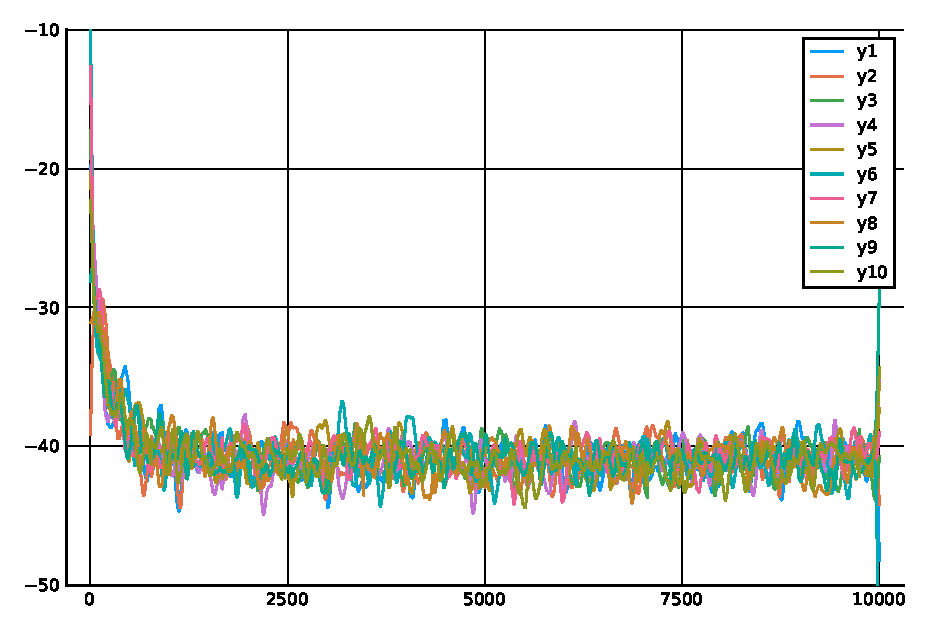
\includegraphics[width=\linewidth]{figuras/err2_cg_sparse.eps}
        \caption{}
        \label{fig:err2_cg}
    \end{subfigure}
    \caption{Mean Square Error for 10 evaluations of 4 different sparsification techniques: (a) Novelty Criterion; (b) Coherence Criterion; (c) Gram-Schmidt; (d) Cartesian Grid}
    \label{fig:err2_sparsifications}
\end{figure}

The grid dictionary we peopose here is chosen at design time, which result in different realizations of the input vectors process having similar MSE. Since the MSE of different realizations are similar, stochastic analysies will be more predictive. Cartesian grids \cite{thompson_handbook_1999} are a type of regular grid with their roots in the integer lattice $\mathbb{Z}^M$ \cite{conway_sphere_1993}. This is a simple grid when compared to others like rhombohedric, irregular grids or others based on different coordinate systems. A dictionary based on a Cartesian grid can be defined as the set
\begin{equation}
    \mathcal{D} = \{ \mathbf{r}_i = \rho\mathbf{z}_i\;|\;\rho \in \mathbb{R}, \mathbf{z}_i \in \mathbb{Z}^M \},\label{eq:grid}
\end{equation}
where $\rho$ is the grid parameter and is the only parameter needed to define it. This means that we have (only) one more parameter to choose in the design of the filter. The index $i$ is in the range $\{1, 2, \dots, N\} $ and the cardinality of the dictionary $|\mathcal{D}| = N$ depends on both the input set $\mathcal{X}$ and the grid parameter.

Some kernels and their parameters are better suited than others when using a Cartesian grid as a dictionary. Radial basis functions \cite{buhmann_radial_2003,scholkopf_learning_2002}, that depend on the distance between points, are good choices since we are choosing exactly the localization of these points. Other kernels with the form $f(.-.)$ are also good choices for the same reason.
% Kernels that depend on other factors, for example, polynomial kernels \cite{scholkopf_learning_2002} that depend on inner product of their variables, are not good choices since the evaluation of the kernel with two vectors that are close but orthogonal as arguments will have a low value.

\section{Kernel Functions and their characteristics}

Three kernel functions were chosen for this work because of their characteristics: 

\subsection{Gaussian Kernel}

The Gaussian kernel 
\begin{equation}
    \kappa(\mathbf{x},\mathbf{y}) = e^{-\frac{||\mathbf{x} - \mathbf{y}||^2}{2\sigma^2}}
\end{equation}
is the most used kernel in the literature of kernel adaptive filters \cite{principe_kernel_2010} because of its approximation properties. It is a normal kernel, which means that 
\begin{equation*}
  \kappa(\mathbf{x},\mathbf{x}) = 1, \forall \mathbf{x} \in \mathcal{X},  
\end{equation*}
and this is its maximum value. It is also a radial basis function, which means that
\begin{equation*}
    \kappa(\mathbf{x},\mathbf{y}) = \phi(||\mathbf{x} - \mathbf{y}||),
\end{equation*}
that is, it is a function of the distance between its arguments. 
We can see the gaussian kernel as the product of many functions, each in one dimension as
\begin{equation}
    e^{-\frac{||\mathbf{x} - \mathbf{y}||^2}{2\sigma^2}} = e^{-\frac{\sum_{i=1}^{M}(x_i-y_i)^2}{2\sigma^2}} = \prod_{i=1}^{M}e^{-\frac{(x_i-y_i)^2}{2\sigma^2}},
\end{equation}
which is known as a tensor product of functions \cite{boor_box_1993}.
The Gaussian kernel has the universal approximation characteristic \cite{steinwart_influence_2002}, which is proved using the Stone-Weierstrass theorem \cite{rudin_functional_2007}. 
% The Stone-Weierstrass theorem \cite{rudin_functional_2007} states that 
% \begin{theorem}
%     (Stone-Weierstrass theorem) Let $(\mathbf{X,d})$ be a compact metric space and $\mathbf{A}(\mathbf{X})$ an algebra of functions. Then $\mathbf{A}(\mathbf{X})$ is dense in $\mathbf{C}(\mathbf{X})$ (the set of continuous functions whose domain is $\mathbf{X}$) if
%     \begin{enumerate}
%         \item for all $x \in \mathbf{X}$, there is an  $f(.) \in \mathbf{A}(\mathbf{X})$ so that $f(x)\neq0$ and
%         \item for all $x,y \in \mathbf{X}$, with $x \neq y$, there is an $f(.)$ so that $f(x) \neq f(y)$.
%     \end{enumerate}
% \end{theorem}
Universal approximation is a characteristic of some sets of functions that, under certain conditions, are dense in another larger set, that is, given a member of the larger set, there is a member of the smaller set that is arbitrarily close to that member. The Stone-Weierstrass theorem guarantees that the set of linear combinations of gaussians is dense in the set of continuous functions.

Despite all of these good characteristics, the Gaussian kernel has a bad one: its support is equal to its domain. The support of a function whose domain is the set $\mathcal{X}$ is defined as \cite{rudin_functional_2007}
\begin{equation}
    \operatorname{supp}_{f(.)} = \{ \mathbf{x} \in \mathcal{X} | f(\mathbf{x}) \neq 0 \},
\end{equation}
but the Gaussian kernel is nowhere equal to zero. Because of this, when using the Gaussian kernel in a kernel adaptive filter, we need $N$ (the number of points in the dictionary) evaluations of the kernel function in each iteration. This means that the greater $N$, the greater the computational power needed. In the case of a dictionary on a Cartesian grid, this translates to the lower $\rho$ in \eqref{eq:grid}, the greater $N$ and so the larger the computational power.

\subsection{Tensor Product of Sincs}

% The Sinc function 
% \begin{equation}
%     \operatorname{sinc}(x) = \begin{cases}
%         \frac{\sin{\pi x}}{\pi x} \quad if \quad x \neq 0\\
%         1  \quad \;\; \quad if \quad x = 0
%     \end{cases}
% \end{equation}
% is well known in the field of signal processing because it is used in sampling theory \cite{oppenheim_discrete-time_2010}. When calculated as

% it is 
The reproducing kernel of an RKHS known as the Paley-Wiener space is given by
\begin{equation}
\kappa(x,y) = \operatorname{sinc}\left( \frac{x-y}{\sigma}\right),
\end{equation}
where the sinc function is
\begin{equation}
    \operatorname{sinc}(x) = \begin{cases}
        \frac{\sin{\pi x}}{\pi x} \quad \text{if} \quad x \neq 0;\\
        1  \quad \;\; \quad \text{if} \quad x = 0.
    \end{cases}
\end{equation}
The members of this space are band-limited functions with a known bandwidth. Sampling theory tells us that this function is capable of regenerating every band-limited function with adequate bandwidth, so that we can assume this to be a universal approximating characteristic for a class of functions.

Since it is a kernel, the product of many of these functions is also a kernel. That is
\begin{equation}
    \kappa(\mathbf{x},\mathbf{y}) = \prod_{i=1}^M \operatorname{sinc}\left( \frac{x_i-y_i}{\sigma} \right),
\end{equation}
is a multivariate kernel. This kernel is also normal, since $\operatorname{sinc}(0) = 1$ and its support is
\begin{equation}
    \operatorname{supp}_{\kappa(\mathbf{x},\mathbf{y})} = \left\{ \mathbf{x},\mathbf{y}\in \mathbb{R}^M \middle| \frac{x_i- y_i}{\sigma} \neq n, n \in \mathbb{Z}^* \right\}
\end{equation}
which means that it is unbounded.

The problem with the support of the Gaussian and tensor product of Sincs kernels motivates us to find another kernel with their desirable characteristics, i.e., normality and universal approximation characteristic, but with a compact support. A kernel with these characteristics is introduced in the next section.

\subsection{Tensor Product of B-Splines}

B-Splines are functions that have been used in interpolation and approximation of functions for decades now \cite{boor_box_1993}. The B-Spline is defined iteratively, starting with the B-Spline of order $0$
\begin{equation}
    b_0(x) = \begin{cases}
            0 \quad \text{if}  \quad x<-\frac{1}{2};\\
            1 \quad \text{if}  \quad -\frac{1}{2} \leq x \leq \frac{1}{2};\\
            0 \quad \text{if}  \quad x \geq \frac{1}{2}.
    \end{cases}
\end{equation}
The other orders are defined as
\begin{equation}
    b_{i+1}(x) = b_i(x)*b_0(x),
\end{equation}
where $*$ is the convolution operation. This means that the B-Spline of order $1$ is
\begin{equation}
    b_0(x) = \begin{cases}
            0 \quad \quad \;\;\; \text{if}  \quad x<-1;\\
            1+x \quad \text{if}  \quad -1 \leq x \leq 0;\\
            1-x \quad \text{if}  \quad 0 \leq x \leq 1;\\
            0 \quad \quad \;\;\; \text{if}  \quad x > 1.
    \end{cases}
\end{equation}
We can see that the support of the B-Spline of order $1$ is the open interval $(-1,1)$.
We can create a positive definite kernel as \cite{scholkopf_learning_2002}
\begin{equation*}
    \kappa(\mathbf{x},\mathbf{y}) = b_i\left( \frac{x-y}{\sigma}\right),
\end{equation*}
where $\sigma$ is its parameter.
A Tensor Product of B-Splines of order $1$ is defined as
\begin{equation}
    B_1(\mathbf{x}) = \prod_{i=1}^{M}b_1(x_i),
\end{equation}
which has a support in the set
\begin{equation*}
    \operatorname{supp}_{B_1(.)} = \underbrace{(-1,1)\times(-1,1)\times \dots\times(-1,1)}_{M \text{factors}}.
\end{equation*}
The Tensor Product of B-Splines of order $1$ kernel
\begin{equation*}
    \kappa(\mathbf{x},\mathbf{y}) = B_1\left( \frac{\mathbf{x} - \mathbf{y}}{\sigma} \right)
\end{equation*}
is a positive definite kernel since it is the multiplication of positive definite kernels \cite{aronszajn_theory_1950}.
It is easy to see that this kernel is of compact support and normal.

To show that this kernel has the universal approximation function, instead of the Stone-Weierstrass theorem, we use Wiener's Tauberian theorem. This theorem states that \cite{wiener_tauberian_1932}
\begin{theorem}
    (Wiener's Tauberian Theorem) Let $f(.) \in \mathcal{L}^2$ (the set of square integrable functions according to the Lebesgue integral) and $f(.+\lambda)$ be the class of translations of $f(.)$. If the Fourier transform of $f(.)$ has zeros that form a set of zero measure, then, given any $g(.) \in \mathcal{L}^2$ and any $\varepsilon_T > 0$, we have a set of coefficients $c_k$ and a set of translations $f(.+\lambda_k)$ such that $g_1(.) = \sum_k c_kf(.+\lambda_k)$ satisfies 
    \begin{equation*}
        \int_{\infty}^{\infty}|g(x) - g_1(x)|^2dx \leq \varepsilon_T.
    \end{equation*}
\end{theorem}

In this case, the set of kernels $\kappa(\mathbf{y},.), \;\; \mathbf{y}\in \mathbb{R}^M$ forms a dense subset of the set of square integrable functions over $\mathbf{X}$, $\mathcal{L}^2$, instead of the set of continuous functions as in the case of the Stone-Weierstrass theorem.

The Tensor product of B-Splines only needs sums and multiplications and no other functions like the exponential as needed to calculate the Gaussian kernel or the sine in sinc. This means that these functions can be easily calculated in an arithmetic logical unit in fixed point arithmetic, without the need for floating point operations, which is suitable for microcontrollers that do not have Floating Point Units.

\section{Orthonormalization procedures}

To create projections of the kernels mapped from the input vectors, we need to create an orthonormal basis from the set of kernels mapped from the vectors in the dictionary. The new basis vectors are linear combinations of the kernels mapped from the vectors of the dictionary
\begin{equation}
    \boldsymbol{\beta}_i = \sum_{j=1}^{M}h_{ij}\kappa(\mathbf{r}_j,.), \mathbf{r}_j \in \mathcal{D}.\label{eq:linearComb}
\end{equation}
We need to guarantee that the inner products of two $\boldsymbol{\beta}_i$, $i=1,2,\dots,N$, are given by
\begin{equation}
    \langle \boldsymbol{\beta}_i, \boldsymbol{\beta}_j \rangle_{\mathbf{B}} = \delta_{ij},\label{eq:KronDelta}
\end{equation}
where $\delta_{ij}$ is the usual Kronecker delta, that is, it is zero if $i \neq j$ and one if $i = j$.
Substituting \eqref{eq:linearComb} in \eqref{eq:KronDelta}, we have
\begin{equation}
    \langle \sum_{\ell=1}^{M}h_{i\ell}\kappa(\mathbf{r}_\ell,.), \sum_{m=1}^{M}h_{jm}\kappa(\mathbf{r}_m,.) \rangle_{\mathbf{B}} = \delta_{ij}.
\end{equation}
Using the linear properties of the inner product and the reproducing property of the kernel, we have
\begin{equation}
    \sum_{\ell=1}^{M}h_{i\ell}\sum_{m=1}^{M}h_{jm}\kappa(\mathbf{r}_\ell,\mathbf{r}_m) = \delta_{ij},
\end{equation}
which can be written in matrix form
\begin{equation}
    \mathbf{H} \mathbf{G} \mathbf{H}^{\top} = \mathbf{I},
\end{equation}
where matrix $\mathbf{G}$ is given by
\begin{equation}
    \mathbf{G} = \left[\begin{matrix}
        \kappa(\mathbf{r}_1,\mathbf{r}_1) & \kappa(\mathbf{r}_1,\mathbf{r}_2) & \dots & \kappa(\mathbf{r}_1,\mathbf{r}_N)\\
        \kappa(\mathbf{r}_2,\mathbf{r}_1) & \kappa(\mathbf{r}_2,\mathbf{r}_2) & \dots & \kappa(\mathbf{r}_2,\mathbf{r}_N)\\
        \vdots & \vdots & \ddots & \vdots\\
        \kappa(\mathbf{r}_N,\mathbf{r}_1) & \kappa(\mathbf{r}_N,\mathbf{r}_2) & \dots & \kappa(\mathbf{r}_N,\mathbf{r}_N)
    \end{matrix}\right],
\end{equation}
and is known as Grammian.
Multiplying by $\left(\mathbf{H}^{\top}\right)^{-1}\mathbf{G}^{-1}$ on the right, we get
\begin{equation}
    \mathbf{H} = \left(\mathbf{H}^{\top}\right)^{-1}\mathbf{G}^{-1},
\end{equation}
where $\left(\mathbf{H}^{\top}\right)^{-1}$ and $\mathbf{G}^{-1}$ exist since both $\{\kappa(\mathbf{r}_i,.)\}$ and $\{\boldsymbol{\beta}_i\}$ are linearly independent.
Multiplying by $\mathbf{H}^{\top}$ on the left, we arrive at
\begin{equation}
    \mathbf{H}^{\top}\mathbf{H} = \mathbf{G}^{-1},\label{eq:HtHG-1}
\end{equation}
so that any $\mathbf{H}$ that orthonormalizes the set of kernels that are mapped by the vectors of the dictionary must satisfy \eqref{eq:HtHG-1}.

One possible $\mathbf{H}$ is obtained using the Cholesky decomposition of $\mathbf{G}^{-1}$, and this corresponds to the Gram-Schmidt orthonormalization procedure since the matrix $\mathbf{H}^{GS}$ obtained in this decomposition is triangular and so one of the $\boldsymbol{\beta}_i$ depends only on one kernel, another of the $\boldsymbol{\beta}_i$ depends on two kernels, and so on.

A second possibility to satisfy \eqref{eq:HtHG-1} is to use 
\begin{equation}
    \mathbf{H}^{LS} = \mathbf{G}^{-\frac{1}{2}},
\end{equation}
where $\mathbf{G}^{-\frac{1}{2}}$ is calculated as
\begin{equation}
    \mathbf{G}^{-\frac{1}{2}} = \mathbf{V}\left[\begin{matrix}
        \frac{1}{\sqrt{\lambda_1}} & 0 & \dots & 0\\
        0 & \frac{1}{\sqrt{\lambda_2}} & \dots & 0\\
        \vdots & \vdots & \vdots & \vdots\\
        0 & 0 & \dots & \frac{1}{\sqrt{\lambda_M}}\\
    \end{matrix}\right]\mathbf{V}^{\top},
\end{equation}
with $\mathbf{V}$ the matrix whose columns are the eigenvectors of $\mathbf{G}$ and $\{\lambda_i\}$ its eigenvelues.
This choice is known in the Quantum Chemistry community as Löwdin Symmetric Orthonormalization \cite{mayer_lowdins_2002}. This procedure minimizes the sum of squared distances \cite{carlson_orthogonalization_1957}
\begin{equation}
    \sum_{i=1}^{M} ||\boldsymbol{\beta}_i - \kappa(\mathbf{r}_i,.)||^2.
\end{equation}

Since $\mathbf{H}^{GS}$ is obtained by the Cholesky factorization of $\mathbf{G}^{-1}$ and $\mathbf{H}^{LS}$ is obtained by calculating the squared root of $\mathbf{G}^{-1}$, we can say that $\mathbf{H}^{GS}$ is the triangular factor of the QR decomposition of $\mathbf{H}^{LS}$ \cite{horn_matrix_2017}.

\begin{figure}
    \centering
    \begin{subfigure}[b]{0.45\linewidth}
        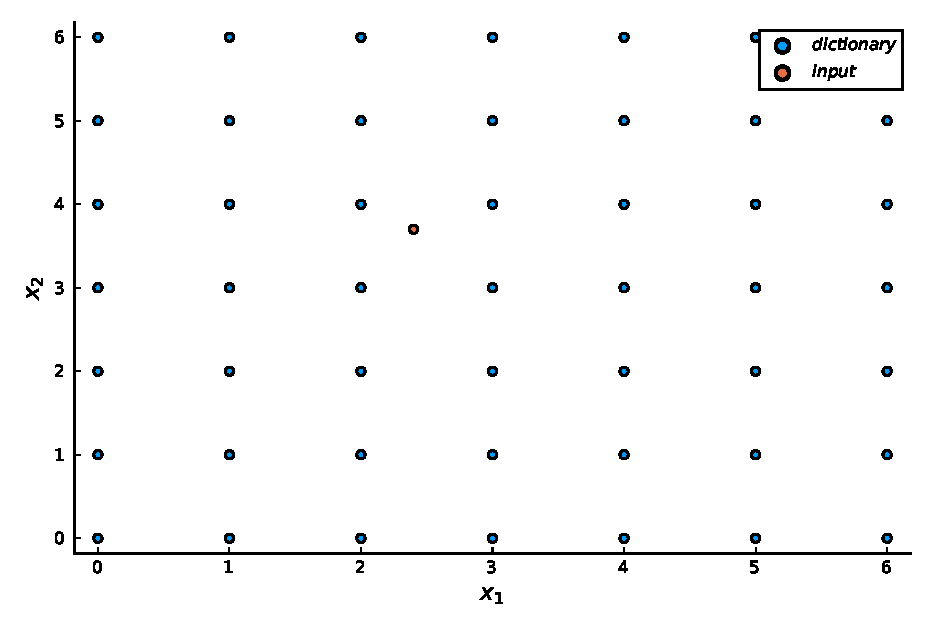
\includegraphics[width=\linewidth]{figuras/scatter_tpbs.eps}
        \caption{}
        \label{fig:tpbs_scatter_1}
    \end{subfigure}
    \begin{subfigure}[b]{0.45\linewidth}
        \includegraphics[width=\linewidth]{figuras/scatter_tpbs_05.eps}
        \caption{}
        \label{fig:tpbs_scatter_05}
    \end{subfigure}
    \caption{Dictionary points and input vector in a Cartesian grid}
    \label{fig:tpbs_scatter}
\end{figure}


Another useful characteristic of the tensor product of sincs and the tensor product of B-Splines of order $1$ is that if we use the parameter of the grid $\rho$ equal to the parameter of the kernel $\sigma$, the Gram matrix is already equal to the identity, meaning that they form an orthonormal basis \cite{horn_matrix_2017}. 
In the case of the tensor product of B-Splines, to compute the output of the filter, we only need to compute the kernels whose dictionary points are the vertices of the hypercube containing the input vector, and not the $N$ kernels mapped from the vectors of the dictionary, because the others are zero. This means that the computational cost (in terms of operations) of the filter is maintained if we use a lower $\rho$. On the other hand, since the number of vectors in the dictionary is bigger with a lower $\rho$, we need more memory to store the filter weights.
This is shown in Figure \ref{fig:tpbs_scatter}. The blue dots represent the dictionary points while the red dot represents the input vector, which is $(2.4,3.7)$. In the system of Figure \ref{fig:tpbs_scatter}\subref{fig:tpbs_scatter_1}, $\sigma = \rho = 1$. In this case, we don't need to compute the kernels corresponding to dictionary points with $x_1 < 1.4$ or $x_1 > 3.4$ since these will result in 0. The same is true for $x_2 < 2.7$ and $x_2 > 4.7$. This leaves us only the kernels corresponding to the points $\mathcal{V}_1 = \left\{(2,3),(3,3),(2,4),(3,4)\right\}$ which are the vertices of the square which contain the input vector.
In the case of the Figure \ref{fig:tpbs_scatter}\subref{fig:tpbs_scatter_05}, $\sigma = \rho = 0.5$, and, using the same reasoning, it is only needed to compute the kernels corresponding to points $\mathcal{V}_2 = \left\{(2,3.5),(2.5,3.5),(2.5,4),(2,4)\right\}$.


\subsection{Example with Gaussian kernels}

In this section, we show an example of orthonormalization of Gaussian kernels using Löwdin Symmetric and Gram-Schmidt techniques. We use nine Gaussian kernels with $\sigma = 1$ and 
centers at $C = \{(0,0),(1,0),(2,0),(0,1),(1,1),(2,1),(0,2),(1,2),(2,2)\}$. 

The matrices obtained for the Gram-Schmidt and for the Löwdin Symmetric techniques are in equations \eqref{eq:H_GS} and \eqref{eq:H_LS} respectively.

% \begin{figure}
%     \begin{subfigure}[b]{\linewidth}
        \begin{equation}
\resizebox{\linewidth}{!}{
$\mathbf{H}^{GS} = \left[
\begin{array}{ccccccccc}
1.0000 & 0.0000 & 0.0000 & 0.0000 & 0.0000 & 0.0000 & 0.0000 & 0.0000 & 0.0000 \\
-0.7629 & 1.2578 & 0.0000 & 0.0000 & 0.0000 & 0.0000 & 0.0000 & 0.0000 & 0.0000 \\
0.4976 & -1.1222 & 1.3526 & 0.0000 & 0.0000 & 0.0000 & 0.0000 & 0.0000 & 0.0000 \\
-0.7629 & -0.0000 & -0.0000 & 1.2578 & 0.0000 & 0.0000 & 0.0000 & 0.0000 & 0.0000 \\
0.5820 & -0.9595 & -0.0000 & -0.9595 & 1.5820 & 0.0000 & 0.0000 & 0.0000 & 0.0000 \\
-0.3796 & 0.8561 & -1.0319 & 0.6259 & -1.4115 & 1.7013 & 0.0000 & 0.0000 & 0.0000 \\
0.4976 & 0.0000 & -0.0000 & -1.1222 & -0.0000 & -0.0000 & 1.3526 & 0.0000 & 0.0000 \\
-0.3796 & 0.6259 & 0.0000 & 0.8561 & -1.4115 & -0.0000 & -1.0319 & 1.7013 & 0.0000 \\
0.2476 & -0.5584 & 0.6731 & -0.5584 & 1.2594 & -1.5179 & 0.6731 & -1.5179 & 1.8296 \\
\end{array}
\right]\label{eq:H_GS}$}
\end{equation}

%     \end{subfigure}    
% \end{figure}
% \begin{figure}
%     \begin{subfigure}[b]{\linewidth}
        \begin{equation}
\resizebox{\linewidth}{!}{
$\mathbf{H}^{LS} = \left[
\begin{array}{ccccccccc}
1.5324 & -0.6442 & 0.2011 & -0.6442 & 0.2708 & -0.0846 & 0.2011 & -0.0846 & 0.0264 \\
-0.6442 & 1.8772 & -0.6442 & 0.2708 & -0.7892 & 0.2708 & -0.0846 & 0.2464 & -0.0846 \\
0.2011 & -0.6442 & 1.5324 & -0.0846 & 0.2708 & -0.6442 & 0.0264 & -0.0846 & 0.2011 \\
-0.6442 & 0.2708 & -0.0846 & 1.8772 & -0.7892 & 0.2464 & -0.6442 & 0.2708 & -0.0846 \\
0.2708 & -0.7892 & 0.2708 & -0.7892 & 2.2997 & -0.7892 & 0.2708 & -0.7892 & 0.2708 \\
-0.0846 & 0.2708 & -0.6442 & 0.2464 & -0.7892 & 1.8772 & -0.0846 & 0.2708 & -0.6442 \\
0.2011 & -0.0846 & 0.0264 & -0.6442 & 0.2708 & -0.0846 & 1.5324 & -0.6442 & 0.2011 \\
-0.0846 & 0.2464 & -0.0846 & 0.2708 & -0.7892 & 0.2708 & -0.6442 & 1.8772 & -0.6442 \\
0.0264 & -0.0846 & 0.2011 & -0.0846 & 0.2708 & -0.6442 & 0.2011 & -0.6442 & 1.5324 \\
\end{array}
\right]\label{eq:H_LS}$}
\end{equation}

%     \end{subfigure}    
% \end{figure}

The functions obtained with the Gram-Schmidt technique are shown in Figure \ref{fig:gs_gaussians} and the ones obtained with the Löwdin Symmetric are shown in Figure \ref{fig:ls_gaussians}.
\begin{figure}[H]
    \centering
    \begin{subfigure}[b]{0.3\linewidth}
        %\input{g_gs_1.tex}
        \includegraphics[width=\linewidth]{figuras/g_gs_1.eps}
        % \caption{Gaussian with center (0,0)}
    \end{subfigure}
    \begin{subfigure}[b]{0.3\linewidth}
        %\input{g_gs_2.tex}
        \includegraphics[width=\linewidth]{figuras/g_gs_2.eps}
        % \caption{Gaussian with center (0,1)}
    \end{subfigure}
    \begin{subfigure}[b]{0.3\linewidth}
        %\input{g_gs_3.tex}
        \includegraphics[width=\linewidth]{figuras/g_gs_3.eps}
        % \caption{Gaussian with center (0,2)}
    \end{subfigure}
    \begin{subfigure}[b]{0.3\linewidth}
        %\input{g_gs_4.tex}
        \includegraphics[width=\linewidth]{figuras/g_gs_4.eps}
        % \caption{Gaussian with center (1,0)}
    \end{subfigure}
    \begin{subfigure}[b]{0.3\linewidth}
        %\input{g_gs_5.tex}
        \includegraphics[width=\linewidth]{figuras/g_gs_5.eps}
        % \caption{Gaussian with center (1,1)}
    \end{subfigure}
    \begin{subfigure}[b]{0.3\linewidth}
        %\input{g_gs_6.tex}
        \includegraphics[width=\linewidth]{figuras/g_gs_6.eps}
        % \caption{Gaussian with center (1,2)}
    \end{subfigure}
    \begin{subfigure}[b]{0.3\linewidth}
        %\input{g_gs_7.tex}
        \includegraphics[width=\linewidth]{figuras/g_gs_7.eps}
        % \caption{Gaussian with center (2,0)}
    \end{subfigure}
    \begin{subfigure}[b]{0.3\linewidth}
        %\input{g_gs_8.tex}
        \includegraphics[width=\linewidth]{figuras/g_gs_8.eps}
        % \caption{Gaussian with center (2,1)}
    \end{subfigure}
    \begin{subfigure}[b]{0.3\linewidth}
        %\input{g_gs_9.tex}
        \includegraphics[width=\linewidth]{figuras/g_gs_9.eps}
        % \caption{Gaussian with center (2,2)}
    \end{subfigure}
    \caption{Functions obtained with the Gram-Schmidt technique}
    \label{fig:gs_gaussians}
\end{figure}

\begin{figure}[H]
    \centering
    \begin{subfigure}[b]{0.3\linewidth}
        \includegraphics[width=\linewidth]{figuras/g_ls_1.eps}
        % \caption{Gaussian with center (0,0)}
    \end{subfigure}
    \begin{subfigure}[b]{0.3\linewidth}
        \includegraphics[width=\linewidth]{figuras/g_ls_2.eps}
        % \caption{Gaussian with center (0,1)}
    \end{subfigure}
    \begin{subfigure}[b]{0.3\linewidth}
        \includegraphics[width=\linewidth]{figuras/g_ls_3.eps}
        % \caption{Gaussian with center (0,2)}
    \end{subfigure}
    \begin{subfigure}[b]{0.3\linewidth}
        \includegraphics[width=\linewidth]{figuras/g_ls_4.eps}
        % \caption{Gaussian with center (1,0)}
    \end{subfigure}
    \begin{subfigure}[b]{0.3\linewidth}
        \includegraphics[width=\linewidth]{figuras/g_ls_5.eps}
        % \caption{Gaussian with center (1,1)}
    \end{subfigure}
    \begin{subfigure}[b]{0.3\linewidth}
        \includegraphics[width=\linewidth]{figuras/g_ls_6.eps}
        % \caption{Gaussian with center (1,2)}
    \end{subfigure}
    \begin{subfigure}[b]{0.3\linewidth}
        \includegraphics[width=\linewidth]{figuras/g_ls_7.eps}
        % \caption{Gaussian with center (2,0)}
    \end{subfigure}
    \begin{subfigure}[b]{0.3\linewidth}
        \includegraphics[width=\linewidth]{figuras/g_ls_8.eps}
        % \caption{Gaussian with center (2,1)}
    \end{subfigure}
    \begin{subfigure}[b]{0.3\linewidth}
        \includegraphics[width=\linewidth]{figuras/g_ls_9.eps}
        % \caption{Gaussian with center (2,2)}
    \end{subfigure}
    \caption{Functions obtained with the Löwdin Symmetric technique}
    \label{fig:ls_gaussians}
\end{figure}
